\documentclass[sigconf]{acmart}
\usepackage{amsmath}
\usepackage{amssymb}
\usepackage{amsfonts}
%\usepackage{graphics}
%\usepackage{curves}
%\usepackage{tikz}
%\usetikzlibrary{backgrounds}
%\usetikzlibrary{snakes} \documentclass{report}
%\usepackage{amsmath}
%\usepackage{amssymb}
%\usepackage{amsfonts}
%\usepackage{graphics}
%\usepackage{curves}
%\usepackage{tikz}
%\usetikzlibrary{backgrounds}
%\usetikzlibrary{snakes}
%\usepackage{setspace}
%\doublespacing
%\usepackage{lscape}
%\usepackage{booktabs}
%\usepackage{longtable}
\usepackage{hyperref}
\usepackage{url}
\usepackage{color}

\author{ABMSPECSIG Group}
\title{Wealth dynamics in the presence of network structure and primitive cooperation}
\bibliographystyle{plain} 
\begin{document}

\maketitle
\begin{abstract}
We study wealth accumulation dynamics in a population of heterogeneously mixed agents with a capacity for a certain primitive form of cooperation enabled by static network structures. Despite their simplicity, the stochastic dynamics generate inequalities in wealth reminiscent of real world social systems even in a fully mixed population. A simple form of cooperation is introduced and is shown to enhance the viability of agents By embedding such dynamics in a network, the impact of social structures on the origins and persistence of inequality can be teased out easily. The models developed here complement traditional modeling approaches based on grid worlds.   

\end{abstract}
\section{Introduction}
In recent years, concerns and debates surrounding wealth inequality and socioeconomic mobility have been one of the few unifying issues dominating the extremely polarized public spheres of the Global North. While economic and political inequality used to be discussed in not so mainstream heterodox economics circles, the contentious discussions on the topic within mainstream economics since the publication of Piketty's book~\cite{piketty2017capital} suggests a lack of consensus about very basic foundational questions like the origins and persistence of economic inequality. Not surprisingly, traditional theories and tools of macro and micro economics are now being diagnosed for their limitations. Simultaneously, insights from related disciplines, along with novel scientific inquiry models not usually associated with traditional econometrics, are being taken more seriously. The work presented here shares this spirit by integrating substantive ideas from anthropology, economic sociology~\cite{granovetter2017society} and urban sociology~\cite{sampson2012great} and using modeling approaches from computational social science~\cite{hedstrom2018}, computational economics~\cite{tesfatsion} and analytical sociology~\cite{hedstrom2011oxford} to understand the origins of inequality in a simple model of wealth dynamics in the presence of social structures.    
% SD: citation for "anthropology," the first element of the last sentence's list? Grief and/or White?

The current work originated in our attempts to incorporate and tease out the effects of social structures in simple models of wealth dynamics in the presence of environmental stochasticity, and a simple form of resource pooling. These models were inspired by our search for analogs of the grid world agent-based models (ABMs) of Friesen and Mudigonda~\cite{srimil} where foraging agents that pool their resources were shown to on-average outperform non-pooling agents. The original model used foraging to mix the population and create opportunities for interaction, and, when certain conditions were met, allowed resource sharing. Our model achieves agent interaction by postulating a static network structure which partially mixes the agents. 

The original model drew its inspiration from historical sociology, in Katz's influential study of middle of 19th century Hamilton, Canada~\cite{katz2013people}. Retaining this original motivation, we draw additional inspiration from economic sociology, in the work of Granovetter~\cite{granovetter2005}; urban sociology, in the work of Sampson~\cite{sampson2002} and others; and in anthropology, in the work on cooperation in small to medium scale societies~\cite{avner1994,white2011kinship}. The geographic and economic scale of the systems, the nature of social actors and time period of interest are all very different from the ones used to develop models of representative agents in macroeconomics~\cite{benhabib2018}, making the similarity between macroeconomic wealth dynamics models and our models not comparable without further justification. Elaborating on the interplay of conceptual and methodological ideas among these disciplines is beyond the scope of this article. Instead, we anchor this work in economic sociology and revisit the insights from the above disciplines in the article's concluding section.

The important role played by social structures or non-economic structures in determining economic outcomes of individuals in a society is not in doubt~\cite{granovetter2005,jackson_rev2017}. Still, in the absence of a unifying foundation for sociology and economics, the full impact of this two-way interpenetration of economic and social structures is demonstrated only on a case-by-case basis. The language of social and economic networks affords a first principle integration by simplifying the non-trivial concept of social and economic structure~\cite{martin_lee} to only dyadic relations. 

As mentioned earlier, macroeconomic models are ill-suited to the study of collective phenomena at an intermediate level. Hence, alternative explanations of aggregate phenomena that match the expressiveness of economic models are required. Analytical sociology~\cite{ch1as_hdbk}, with its emphasis on explanation of collective emergent phenomena using mathematically formulated social mechanisms~\cite{ch2as_hdbk,ch11as_hdbk} anchored at the individual level, is an ideal candidate for this purpose. It is particularly powerful when combined with computational simulation, because when mathematically-formulated models reach even a modest level of complexity, they often become analytically intractable. Simulation \textit{in silico} can yield approximate results for these more complex scenarios, which supplement the exact results reached by traditional methods.

Models constructed here, like those used in scientific inquiry in general, serve a specific purpose. In this work, we construct simple toy models to reproduce certain aspects of non-trivial wealth inequality distributions in the presence and absence of primitive forms of cooperation, clearly delineating the role of network structure in generating wealth inequality. We make no suggestions that these models \textit{explain} the phenomena of interest; we are only interested in constructing the simplest possible models, with no detailed empirical grounding, but with the potential to generate realistic looking inequality distributions. In doing so, we aspire to shed light on the \textit{true} social and economic mechanisms underlying the genesis and persistence of economic inequality. 


% SD: In light of recent discussions, we may want to downplay Gini and up-play the robustness of agents to exogenous shocks.
The phenomenon under scrutiny is the emergence and evolution of economic inequality in societies with non-trivial social structures. The model we use to answer questions surrounding this phenomenon must possess a dynamic model of wealth accumulation, a model of social structure, and a suitably useful measure of inequality. The dynamics are modeled as Brownian noise driven linear dynamical systems, here constant growth rate; the structure is modeled by networks, here random graphs; the measures of inequality used are Gini coefficients, and survival time distributions of agents in response to lack of resources. Although both the dynamical system and the network model are quite well understood, the precise interplay of structure and dynamics produces interesting emergent wealth distributions. To the best of our knowledge, this specific combination of network structure and social dynamics has not been discussed in the computational social science (CSS) or mathematical sociology literature, and we consider this the primary contribution of this work. 

Apart from enabling interactions between social actors, social structures like institutions also shape the form of cooperation and coordination mechanisms. The institutions can take the form of economic institutions, like banks and cooperatives; or the form of norms, like resource-sharing practices in societies. The original SriMil model~\cite{srimil}consists of a simple resource pooling arrangement where aggregates of agents pool their excess wealth in a common institution called ``proto-institutions,'' agreeing to provide this saved resource to individual agents in times of need. The model of resource pooling used in this work is identical to the SriMil model. 

The analysis to be presented in later sections focuses only on homogeneous agents with simple drift-diffusion dynamics on Erd\H{o}s-R\'{e}nyi network models (ER); space constraints unfortunately prevent us from repeating the analysis on other standard \textit{textbook} networks like scale-free and small-world networks. We discuss empirical evidence for the role of social network structures in the concluding section of this paper, motivating the need for more expressive social network models. 


In the next section, we discuss the mathematical formulation of the model. In section 3, we present the analysis of our simulation experiments, summarize key findings and discuss why we chose the \texttt{julia} programming language~\cite{Julia-2017} for our implementation. In section 4, we discuss the limitations of our simple models, extensions to dynamics and networks more expressive than the ones presented here, and planned future work. 

Before discussing our model in greater mathematical detail, we discuss the model qualitatively, contrasting them with more familiar modeling approaches. The model presented here has much in common with models used in social reality inspired models in statistical physics~\cite{redner2001guide}, dynamic process models in network science~\cite{newman2018networks}, and computational social science and agent-based models~\cite{abm_review}; however, our modeling philosophy is somewhere at the interface of agent-based computational economics (ACE)~\cite{tesfatsion} and analytical sociology (AS)~\cite{ch1as_hdbk,ch2as_hdbk}. In ACE, we acknowledge its aspiration to develop bottom-up models of economic systems at all scales but restrain from its enthusiastic use of complex but well-calibrated detailed models of markets and agents~\cite{tesfatsion2017}. In AS, we assent its focus on social mechanisms in explaining social phenomena, but instead rely on simplified mechanisms with few parameters~\cite{ch11as_hdbk} with the specific goal of extracting insights from \textit{stylized} models.       

More specifically, from statistical physics, we borrow the dynamics: diffusion models and associated first-passage time techniques; from network science, we borrow the structural aspects: Erd\H{o}s-R\'{e}nyi network (ER) models; and from non-equlibrium statistical physics, CSS and ACE, we borrow a form of cooperation: the concept of coalescence, institution and coordination. 



\section{Model}
The model of cooperative wealth accumulation constructed here is best thought of as a stochastic interacting particle system infused with economic sociological semantics. The particle evolves according to an one dimensional diffusion process with constant drift and is driven by a Brownian noise with boundary condition at the origin corresponding to particle absorption. After crossing a pre-determined threshold in state space, particles above the threshold follow a protocol and coalesce together. In an ensemble of otherwise identical particles, a given particle may coalesce with a subset of other particles. This mixing characteristic is encoded via a graph. Both the conjoined particles and individual particles die upon crossing the origin. This model of interacting diffusing particles can be provided with substantive semantics as follows. 

%Might be nice to put a nice table here 
The one dimensional state space of the particle is identified with the wealth of an social actor (agent). We consider a homogeneous population where all agents are required burn their wealth at a constant specified rate in order to survive. In addition, the agents all gain wealth at a constant rate. The resource draining rate and the resource gaining rate are additive and constitute the drift of the diffusion process. The environmental contingency is modeled by a Brownian noise of a specified intensity. Upon crossing a specific wealth threshold, agents can coalesce to form a cooperative unit deciding to pool their resources and their environmental contingencies into a single unit which we call a \textit{proto-institution} (proto). The mixing characteristic of this ensemble is the social network (here ER model).          



~\cite{redner2001guide} ~\cite{rv}  ~\cite{wilhite} ~\cite{arthur} 




\subsection{Implementation}
%Stephen thinks that a subsection of the Model section should be about the
%simulation code. It won't be long; just enough to explain how the mathematical
%model just described is represented and executed in Julia, including some
%answers to non-obvious questions that arise when considering implementation.

\section{Analysis}
%% (Separate analysis.tex file, so all images are in a separate file.)

First, we verify that the simulation's output matches obviously expected
results. Then, we investigate aspects of its behavior which are not computable
analytically in order to discover important consequences of the model.


\subsection{Verification}

\subsubsection{Single simulation runs}

For a sensible range of parameter settings, the life history of a single
simulation run follows an expected pattern. Assuming a positive growth rate
(\textit{i.e.}, salary > metabolic rate), each agent's wealth rises unsteadily
during stage 1, until eventually the first pair of neighboring agents who each
reach the threshold form a proto-institution. Throughout stage 2, these agents
contribute all wealth in excess of the threshold to that proto, and so their
proto's balance rises unsteadily while their personal wealth remains at the
constant threshold. Meanwhile, the other agents also reach the threshold at
various points in time, and also form or join protos, until every non-isolate
(that is, every node with at least one neighbor) is a member of a proto. Stage
3 (the starvation period) then commences, with isolates drawing on a greater
personal wealth than the non-isolates. When an isolate reaches zero wealth, it
dies; when a non-isolate reaches zero, it draws from its (shared) proto balance
until that too, reaches zero, and it dies.

\begin{figure}[ht]
\centering
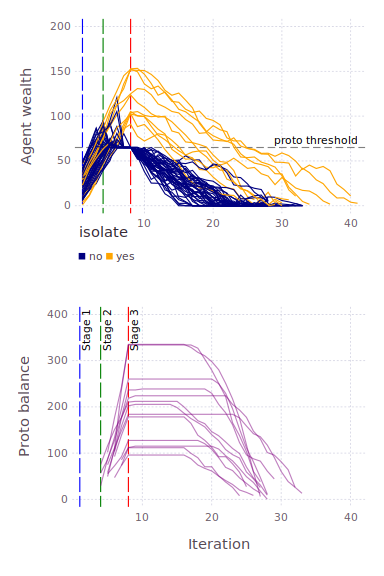
\includegraphics[width=\columnwidth]{figures/sampleLifeHistory.png}
\caption{A single run of the simulation, with $\lambda$=2. Each of 50 nodes is
given an initial wealth of 50 units, a regular income distributed as
$\sim\mathcal{N}(20,5)$, a metabolic rate of 5, and a proto threshold of 65.}
\label{fig:singleRun}
\end{figure}

This history can be seen in Figure~\ref{fig:singleRun}. The top plot depicts
agent wealth at every iteration, and the bottom plot shows the balances of the
protos at the same points in time. (No protos exist until stage 2, by
definition.) Note that the isolates (orange lines) never form protos, and
therefore begin the starvation stage with a higher personal wealth to draw
from.


\begin{figure}[ht]
\centering
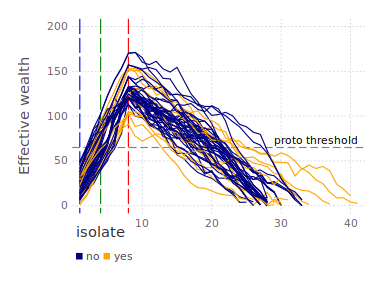
\includegraphics[width=\columnwidth]{figures/sampleEffectiveHistory.png}
\caption{The same simulation run as Figure~\ref{fig:singleRun}, but this time
depicting each agent's \textit{effective} wealth (its personal wealth plus its
share of its proto's wealth, if any).}
\label{fig:effectiveWealthSingleRun}
\end{figure}

Figure~\ref{fig:effectiveWealthSingleRun} shows the same information in another
way: instead of plotting each agent's \textit{personal} wealth (as in the top
plot of Figure~\ref{fig:singleRun}, we show its \textbf{effective wealth},
defined as the sum of its personal wealth and its ``share'' of its proto's
wealth (if any). After all, contributions that a proto's members make to its
balance are available to those members in times of need; therefore, a fair
comparison between isolates and non-isolates should take this into account.
From the figure, it can be seen that isolates no longer have a systematic
advantage (as they appeared to in Figure~\ref{fig:singleRun}.

We verified that changes to basic parameters all have the expected effect:
lowering the initial wealth delays the onset of stage 2; a higher $\sigma^2$
for the income distribution makes the lines less jagged; a higher metabolic
rate hastens extinction; \textit{etc.}


% Note that the empty graph can't really be shown because stages 2 and 3 have
% no well-defined meaning in that case.

% Show Gini plot, null hypothesis, "this is why it doesn't matter"

% Show different levels of white noise intensity relative to growth rate
%     (salary - metabolic rate)


\subsubsection{Parameter sweeps}

% Gini coefficient (pre-stage-3) decreases with λ

\subsection{Findings}

% Wealth histogram is steady ?

% Which is better strategy: to form protos when possible, or not?


\section{Conclusion and Future Work}


%%%%%%%%%%%%%%%%%%%%%%%%%%%%%%%%%%%%%%%%%
%%%Things that could be discussed here but is redundant if we are running out of words 
%The general idea is to discuss how/why social networks matter wealth accumulation dynamics. We have references from anthropology. We have references in economic sociology(jackson).Sampson's work and Venkatesh's work can be used when talking about urban poverty and urban sociology. Discuss how in economics, wealth accumulation dynamics are mostly discussed at the macroeconomic level. In this sense, this work (and the work presented last year) are novel in this regard.  

%% Sampson's work seem to be crucial for making the claim that social structures and neighborhood effects are important determinants of economic outcomes. 

% Wealth accumulation models all start from fancy macroeconomic models and may not be well suited for studying wealth accumulation processes under poverty where high level of stochasticity seem to matter. 

%While we are interested in more sophisticated models, we are more interested in extracting the effects of social network structure in simple models of cooperative wealth accumulation. The proto-institution is definitely borrowed from SriMil. In order to study more elaborate and economically rigorous wealth dynamics, we need to be able sort of the effects of network structure in simple stylized network models. The work on ER models is expected to be first of our analysis. Eventually, we plan to get to more realistic wealth accumulation models of interest to economists but for now this is all we have.  

%In Katz's book, the differing life histories of individuals in Hamilton, Canada suggest that luck played a role in deterministic life outcomes. Katz argues that social mobility makes sense only in the context of social structure

%Katz's chapter 2. His main argument there is that the structure of inequality represent in Hamilton, Canada is representative of inequality present in all other north American cities of that era. The persistence of inequality can be see in the persistence of four kinds of social structures. 1) occupational structure, 2) division of wealth and proportion of the wealthy, 3) social and demographic identity of different economic ranks, and 4) distance between people of different socio-economic ranks or social stratification. He talks about persistence of networks of wealth and power. Points out strong interconnection between property, political power and social status. Argues that economic stratification and its crystallization leads to crystallization of social and other subjective stratifications.  



%%%%%%%%%%%%%%%%%%%%%%%%%%%%%%%%%%%%%%
%%%% This one is really important and top priority for use as a zoomed out conclusion 
%what kinds of real world systems are we talking about?This section should write itself. Just a brief discussion of phase 2+ and integration with spescape should suffice 
%%%% ERGM, SBM and LNM are good next steps 
%%%%% Use anthropology references to motivate more expressive models 
\cite{power2018cooperation,power2018}

\cite{koster2019,koster2014,koster2015,bogerhoff2015}

\cite{smith2019,nolin2012}


%%%% 

%%%%%%%%%%%%%%%%%%%%%%%%%%%%%%%%%
%I am actually confused about whether such a purely preliminary work can say antyhing about the real world. Do we really want to say anything at all about the real world. What can ER graphs say about the real world?  

%We conclude by discussing features of social processes and mechanisms argued for by both Sampson and Katz that are currently not present in the model but important and part of the vision for where our model is headed. 

%We also include the goal of seamlessly going from a model with no geography to a model with geography. 

% I am moving the discussion of connections to anthropology to this section 


\bibliography{ref_cssa19}
\end{document}
% this line is for Stephen's purposes only:
% vim:textwidth=99999
